\documentclass[preprint]{aastex}
\usepackage{amssymb,amsmath,verbatim}
\title{Removing the impact of the balun in reflectometry measurements for HERA EoX project.}
\author{Aaron Ewall-Wice}
\begin{document}
\maketitle
\section{The S-matrix description of the balun.}
We first discuss how measurements of the S-parameters of the three unbalanced ports of a balun may be used to determine and undo its impact on measurements of the differential S-parameters of an antenna. A balun may be described as a three port system with the unbalanced port numbered on and the balanced port formed from two unbalanced ports which we will label $2$ and $3$. Incoming waves at each port are related to outgoing waves by the S-matrix.
\begin{equation}\label{eq:SMatrix}
\begin{pmatrix} b_1 \\ b_2 \\ b_3 \end{pmatrix} = \begin{pmatrix} S_{11} & S_{12} & S_{13} \\
				S_{21} & S_{22} & S_{23} \\
				S_{31} & S_{32} & S_{33} \end{pmatrix} \begin{pmatrix} a_1 \\ a_2 \\ a_3 \end{pmatrix}
\end{equation}
or
\begin{equation}
{\bf b} = \boldsymbol{\mathsf{S}} {\bf a}
\end{equation}
Since we are ultimately attempting to measure the S-parameters of the differential antenna, it is convenient for us to work in the differential and common-mode basis for ports $2$ and $3$.  We define the differential and common mode incoming and outgoing waves as 
\begin{align}
a_c &= \frac{1}{\sqrt{2}} \left(a_2 + a_3\right)\\
a_d &=\frac{1}{\sqrt{2}} \left(a_2 - a_3 \right) \\
b_c &= \frac{1}{\sqrt{2}} \left(b_2 + b_3 \right)\\
b_d &= \frac{1}{\sqrt{2}} \left(b_2 - b_3 \right)
\end{align}
The transformation matrix between the un-balanced and balanced basis is given by the matrix
\begin{equation}
{\boldsymbol{\mathsf{M}}}=\frac{1}{\sqrt{2}}\begin{pmatrix} 1 & 0 & 0 \\ 0 & 1 & 1 \\ 0 & 1 & -1\end{pmatrix}
\end{equation}
The S-matrix in this basis may be expressed as the transformation 
\begin{equation}\label{eq:SMatrixDifferential}
\begin{pmatrix} b_1 \\ b_c \\ b_d \end{pmatrix} = \begin{pmatrix} S_{11} & S_{1c} & S_{1d} \\
				S_{c1} & S_{cc} & S_{cd} \\
				S_{d1} & S_{dc} & S_{dd} \end{pmatrix} \begin{pmatrix} a_1 \\ a_c \\ a_d \end{pmatrix}
\end{equation}
or
\begin{equation}\label{eq:Transformations}
{\bf b^\prime} = \boldsymbol{\mathsf{S}^\prime} {\bf a^\prime} \text{ where }
{\bf b^\prime} = \boldsymbol{\mathsf{M}} {\bf b} \text{ , }
{\bf a^\prime} = \boldsymbol{\mathsf{M}} {\bf a} \text{ , and }
\boldsymbol{\mathsf{S}^\prime} = \boldsymbol{\mathsf{M}} \boldsymbol{\mathsf{S}}\boldsymbol{\mathsf{M}}^{-1}
\end{equation}
We can apply the matrix transformation in the third equation of \ref{eq:Transformations} to derive the differential S-matrix of our balun. Here is the mathematica code
\begin{verbatim}
Mmatrix = {{1, 0, 0}, {0, 1/Sqrt[2], 1/Sqrt[2]}, {0, 1/Sqrt[2], -1/
    Sqrt[2]}};
Smatrix = {{s11, s12, s13}, {s21, s22, s23}, {s31, s32, s33}};
MatrixForm[FullSimplify[Mmatrix.Smatrix.Inverse[Mmatrix]]]
\end{verbatim}
which gives us
\begin{equation}\label{eq:SMatrixBal2uBal}
\begin{pmatrix} S_{11} & S_{1c} & S_{1d} \\
				S_{c1} & S_{cc} & S_{cd} \\
				S_{d1} & S_{dc} & S_{dd} \end{pmatrix} = \begin{pmatrix} S_{11} & \frac{S_{12}+S_{13}}{\sqrt{2}} & \frac{S_{12}-S_{13}}{\sqrt{2}} \\ \frac{S_{21}+S_{31}}{\sqrt{2}} & \frac{1}{2} \left( S_{22}+S_{23}+S_{32}+S_{33}\right)& \frac{1}{2}\left(S_{22}-S_{23}+S_{32}-S_{33} \right) &\\
\frac{S_{21}-S_{31}}{\sqrt{2}} & \frac{1}{2}\left(S_{22}+S_{23}-S_{32}-S_{33}\right) & \frac{1}{2} \left(S_{22} - S_{23} - S_{32} + S_{33}\right) \end{pmatrix}
\end{equation}
Having measured the unbalanced S-parameters of the balun, we may obtain the differential and common mode S-parameters from the single-port S-parameters with equation~\ref{eq:SMatrixBal2uBal}.
\section{Measurements of the balun as a three-port system}\label{sec:BalunMeasurements}
\section{Characterization of the balun using back-to-back baluns.}
If one assumes that balun has good common-mode rejection, it is possible to characterize the balun through a two-port measurement of two baluns attached back-to-back on their differential port. In this measurement, the VNA has the RF-out arm attached to the unbalanced port of one balun and the RF-in arm on the other. The VNA measures both the $S_{11}^\prime \equiv R^m$ of the back to back baluns and $S_{21}^\prime \equiv T^m$. We illustrate the path of an inserted signal at the unbalanced port of the first balun in Fig.~\ref{fig:BackToBackBaluns}. 
\begin{figure}
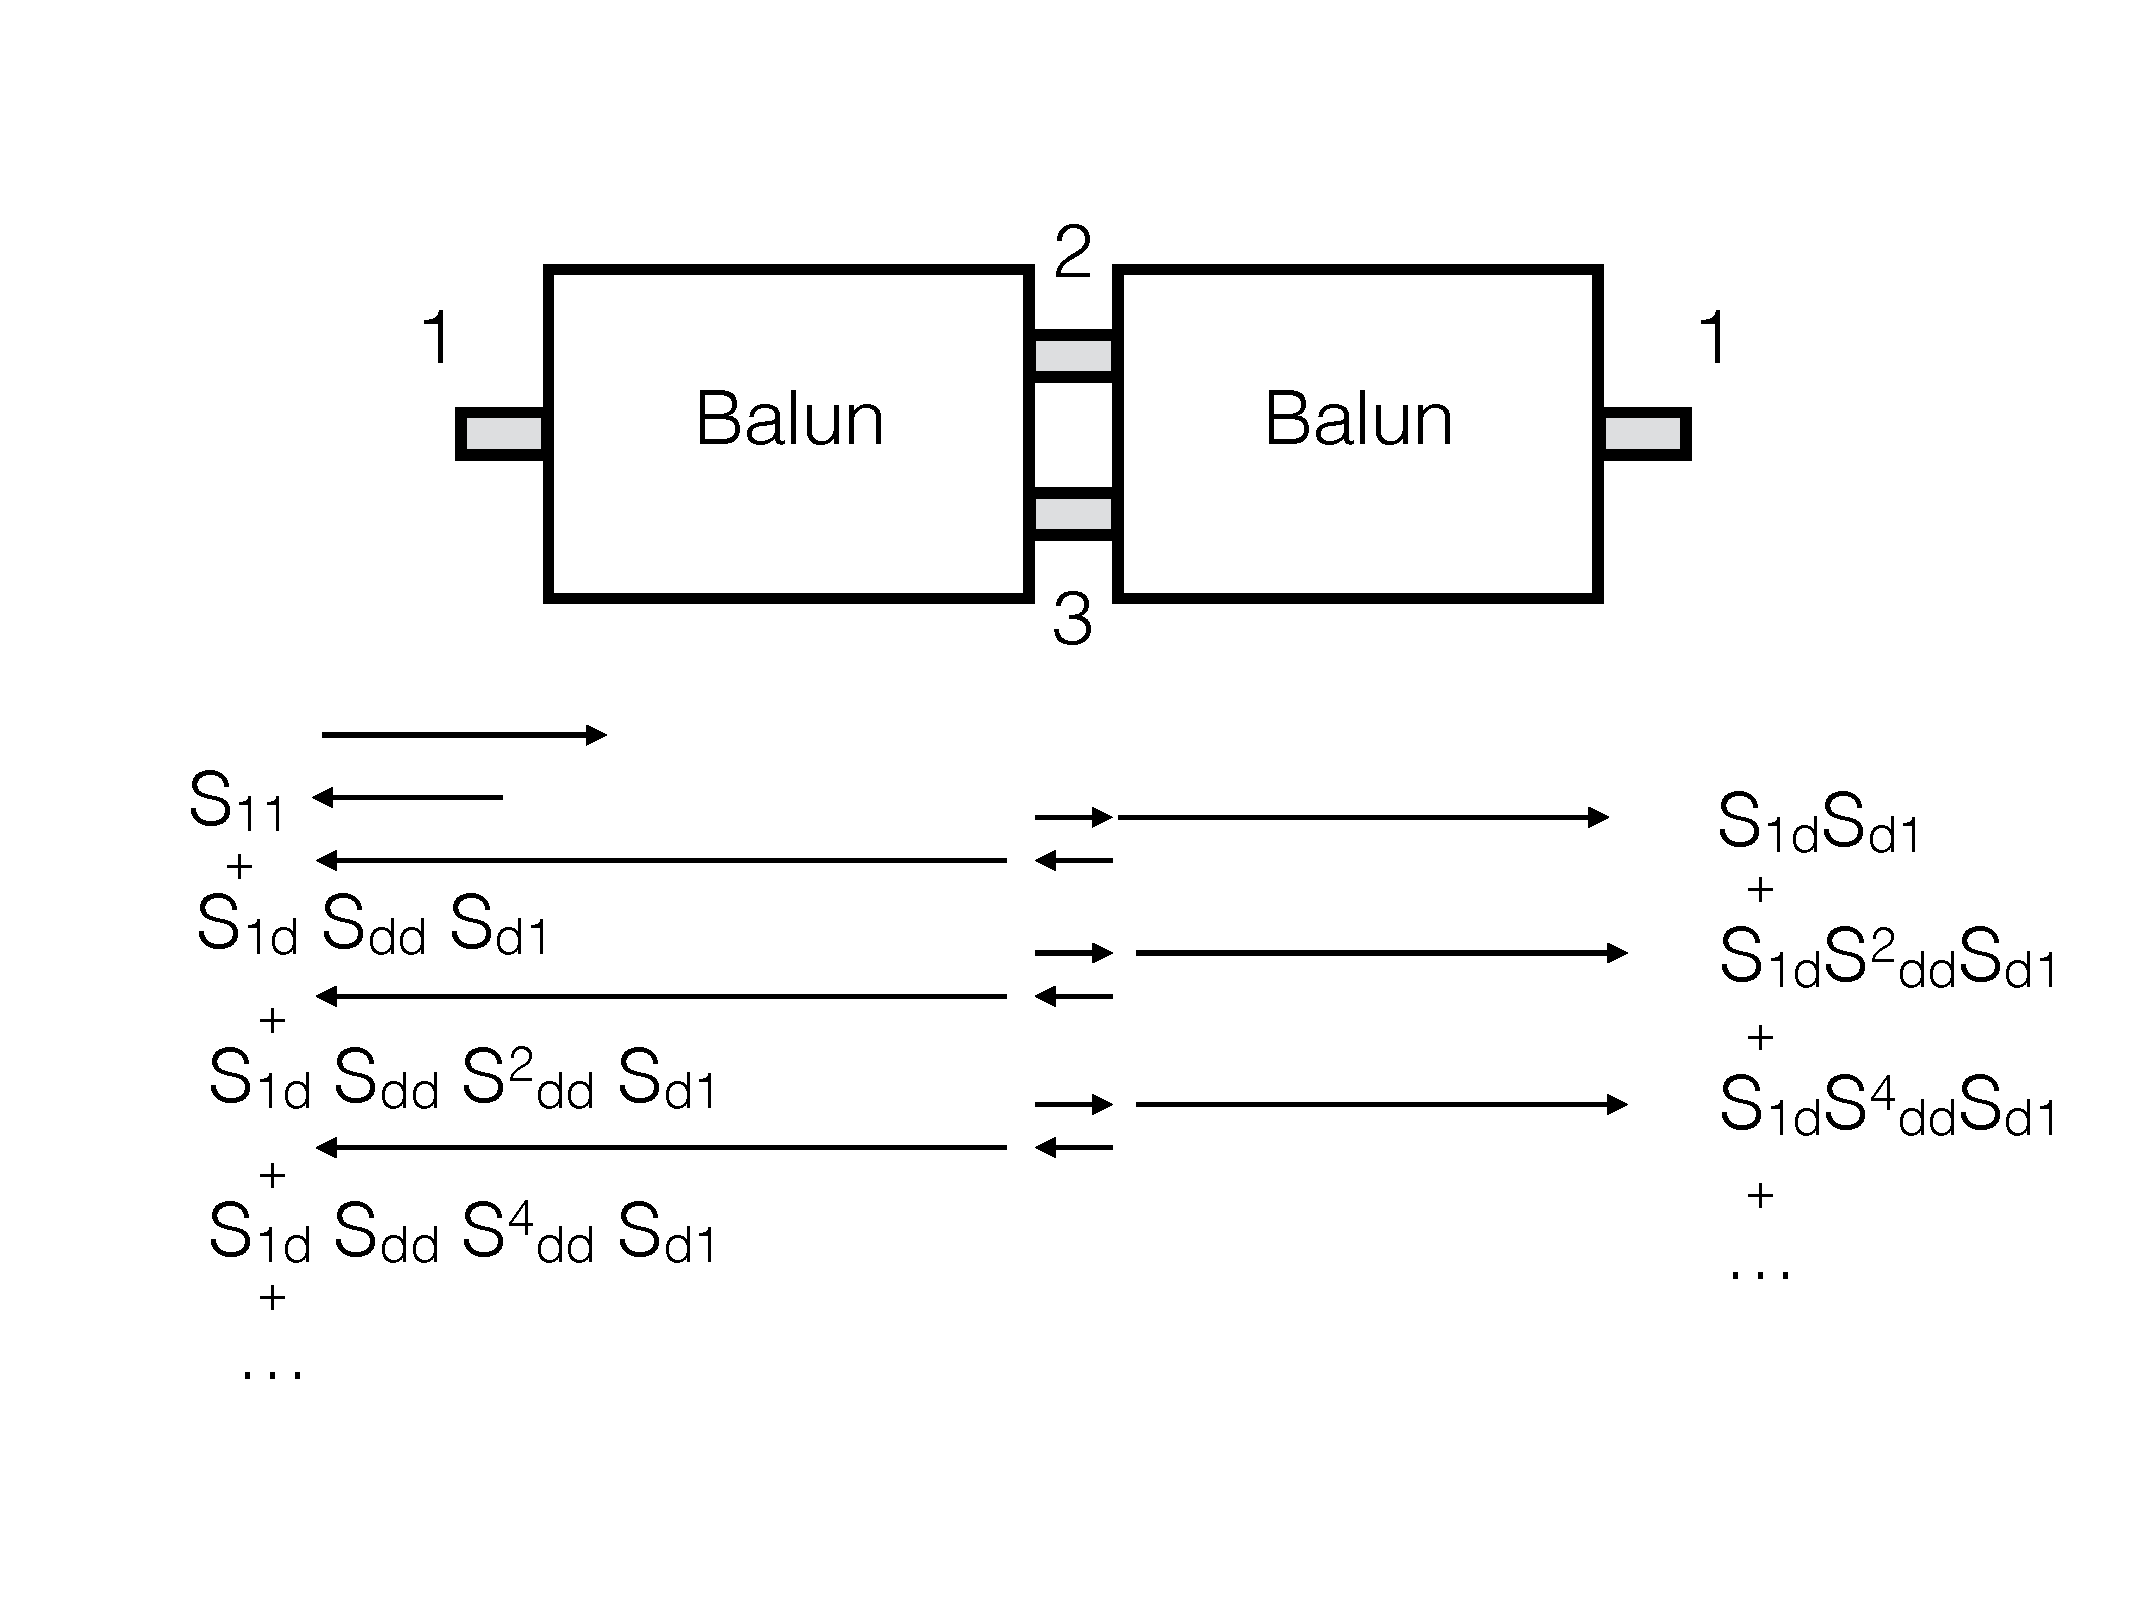
\includegraphics[width=\textwidth]{back_to_back_baluns.pdf}
\caption{An illustration of the wave components arising at the input and output unbalanced ports of back-to-back baluns which give rise to equations~\ref{eq:ReflectionBackToBack} and \ref{eq:TransmissionBackToBack}}
\end{figure}
The reflected signal used to determine $\Gamma_m$ is equal to the sum of the initial reflection off of $S_{11}$ plus the component of the signal that is transmitted to the interface between the two baluns, is reflected back, and transmitted back out of port-1, picking up a factor of $S_{1d} S_{dd} S_{d1}$. A component of this signal is not transmitted but is rather re-reflected within the balun-balun interface, picking up an additional factor of $S_{dd}^2$ before being transmitted back and re-reflected. The resulting series of reflection gives us 
\begin{align}
R^m &= S_{11} + S_{1d}S_{dd}S_{d1} + S_{1d}S_{dd} S_{dd}^2 S_{d1} + \dots + S_{1d} S_{dd} S_{dd}^{2m} S_{d1} \nonumber \\
&= S_{11} + \frac{S_{1d} S_{dd} S_{d1}}{1-S_{dd}^2}\label{eq:ReflectionBackToBack}
\end{align}
The transmitted signal used to determine $T^m$ results from a component that is transmitted through the first balun and the second balun, $S_{1d}S_{d1}$ plus a component that is transmitted through the first balun, reflected between the baluns, and re-transmitted, picking up a factor of $S_{dd}^2$, and the sum of re-reflected components, which each pick up a factor of $S_{dd}^{2m}$, for $m$ re-reflections. This sums to be 
\begin{align}
T^m &= S_{1d}S_{d1} + S_{1d}S_{dd}^2S_{d1} + \dots + S_{1d} S_{dd}^{2m} S_{d1} \nonumber \\
 & = \frac{S_{1d}S_{d1}}{1-S_{dd}^2}\label{eq:TransmissionBackToBack}
\end{align}
If we measure $S_{11}$ using the three-port technique, we can also subtract it to determine $S_{dd}$. 
\begin{equation}
S_{dd} = \frac{R^m - S_{11}}{T^m}
\end{equation}
We can also detrmine $S_{1d} S_{d1}$ 
\begin{equation}
S_{1d}S_{d1} = \frac{\left(R^m-S_{11}\right)\left(1-S_{dd}^2\right)}{S_{dd}}
\end{equation}
\section{The impact of the balun on antenna reflectometry.}
\subsection{Assuming no common-mode reflections}
To simplify things, we assume that $S_{12}=-S_{13}$ and $S_{21}=-S_{23}$ (we check this in section~\label{sec:BalunMeasurements}) so that $S_{1c}=S_{c1}=0$. Our goal is to determine $\Gamma$, the differential reflection coefficient of the antenna. These assumptions on the balun can also be relaxed as long as the antenna itself has negligible reflection coefficient $\Gamma_c = 0$. Thus the assumptions of this analysis are $S_{1c}=S_{c1}=0$ or $\Gamma_c = 0$. 

The reflection coefficient we measure, we shall call $\Gamma^m$. Here we compute $\Gamma^m$ in terms of the balun's $S-parameters$ and $\Gamma$. We consider an input wave $a_m$ from the VNA on the unbalanced-port $1$ of the balun. The VNA measures $b_m$ at the output of port-1 and divides by $a_m$ to determine $\Gamma^m$. $b_m$ is contributed to from an initial reflection off of port-$1$ given by the $S_{11}$ of the balun along components of the input wave that are transmitted through the balun to the antenna and subsequently reflected.
\begin{equation}
b_m =  S_{11} a_m + \text{subsequent reflections}.
\end{equation}
What are these subsequent reflections? The component of the wave that is not immediately reflected at port-1 of the balun is transmitted into both the common and differential mode. We will ignore common-mode for now so that a signal is incident from the balun onto the antenna terminals that is given by 
\begin{equation}
 S_{d1} a_m
\end{equation}
 This wave is reflected off of the antenna and back onto the differential port of the balun with a factor of the $\Gamma$ acquired. A component of this  wave is transmitted into port-1 with a total complex amplitude of 
 \begin{equation}
 S_{d1} \Gamma S_{1d} a_m
 \end{equation}
 so that our total reflected wave has an amplitude of 
 \begin{equation}
 b_m = S_{11} a_m + S_{d1} \Gamma S_{1d} a_m + \dots 
 \end{equation}
 we are not done because we have still not included the component of the wave that was reflected off of the antenna that did not transmit through the balun to port-1. This component is re-reflected back onto the antenna and returns to the differential port of the balun with an additional factor of $ \Gamma S_{dd}$ some of it will be transmitted to port-1 with a factor of $S_{1d}$ and another component will be re-reflected to pick up another factor of $ \Gamma S_{dd}$ before undergoing the same partial transmission and re-reflection. The sum of these reflections between the differential balun-port and the antenna terminals adds an infinite geometrical sum to $b_m$.
 \begin{align}
 b_m &= S_{11} a_m + S_{d1} \Gamma S_{1d} a_m + S_{d1} \Gamma S_{dd} \Gamma S_{d1} a_m + \dots + S_{d1} \Gamma \left(\Gamma S_{dd}\right)^m S_{1d} a_m \nonumber \\
 &= S_{11} a_m + \frac{S_{d1} \Gamma S_{1d}}{1-S_{dd}\Gamma} a_m 
 \end{align} 
 Thus the measured reflection coefficient is 
 \begin{equation}\label{eq:MeasuredReflections}
\Gamma^m = S_{11} + \frac{{S_d1}\Gamma S_{1d}}{1-S_{dd} \Gamma}
 \end{equation}
 The antenna can be de-imbedded from the balun by solving equation~\ref{eq:MeasuredReflections} for $\Gamma$. 
 \begin{equation}
 \Gamma = \frac{\Gamma^m - S_{11}}{S_{1d}S_{d1} + S_{dd}\left(\Gamma^m-S_{11}\right)}
 \end{equation}
 Both $S_{1d}S_{d1}$ and $S_{dd}$ can be obtained either through back-to-back balun measurements ore the three-port balun technique. 
\end{document}

